\chapter{Testing}
\label{ch:testing}

\section{Overview}

This chapter describes the implementation of the \ref{ch:methodology} chapter's methodology through the usage and analysis of a data set provided by Arcos \cite{arcos}. 



- descrizione dei dati originali, percentuali
- descrizione dei viaggi, percentuali
- heatmap
- 

\subsection{The original Dataset}
The source dataset selected to carry out testing of the described methodology is as mentioned composed of AIS messages.
Nel dettaglio, si tratta di messaggi provenienti da navi che hanno attraversato la zona artica e dintorni negli anni 2019, 2020 e 2021.
In numbers:
\begin{itemize}
\item 95,294,750 AIS messages;
\item 10,058 different vessels;
\item 6,777 segments generated.
\end{itemize}


\subsection{PCA, a graphical clusters rapresentation technique}

In order to a get an idea of the clusters from a graphical point of view, a \textbf{dimensionality reduction} procedure was used: \textbf{Principal Component Analysis}.
PCA has the task of reducing an input space with n dimensions into a space with smaller number of dimensions.
Since the goal in this case was to obtain a graphical representation of the clusters, the number of components to which the 7 input components were reduced was \textbf{2}.

What DBSCAN produces in this context is a dataset of clusters and all the possible information to locate in a 7-dimensional space (the 7 chosen features, indeed) the trips that were given to it as input.
More precisely, each pathway is classified as:
\begin{itemize}
\item \textbf{Core Point} if it is a point that contributed to the cluster expansion, as described in the section; \ref{subsec:dbscan-example}
\item \textbf{Non-Core Point} if it is a point that has not contributed to cluster expansion;
\item \textbf{Outlier} if for some reason the algorithm did not include the trip in any generated cluster.
\end{itemize}

Of course, it is very complicated to depict a space with a number of dimensions greater than 2, so the result of this DBSCAN would be difficult to represent.

Using the Principal Component Analysis (PCA) technique with two components, it has been possible to graphically represent the obtained clusters despite the 7-dimensions space of the original data.

\begin{figure}[H]
    \centering
    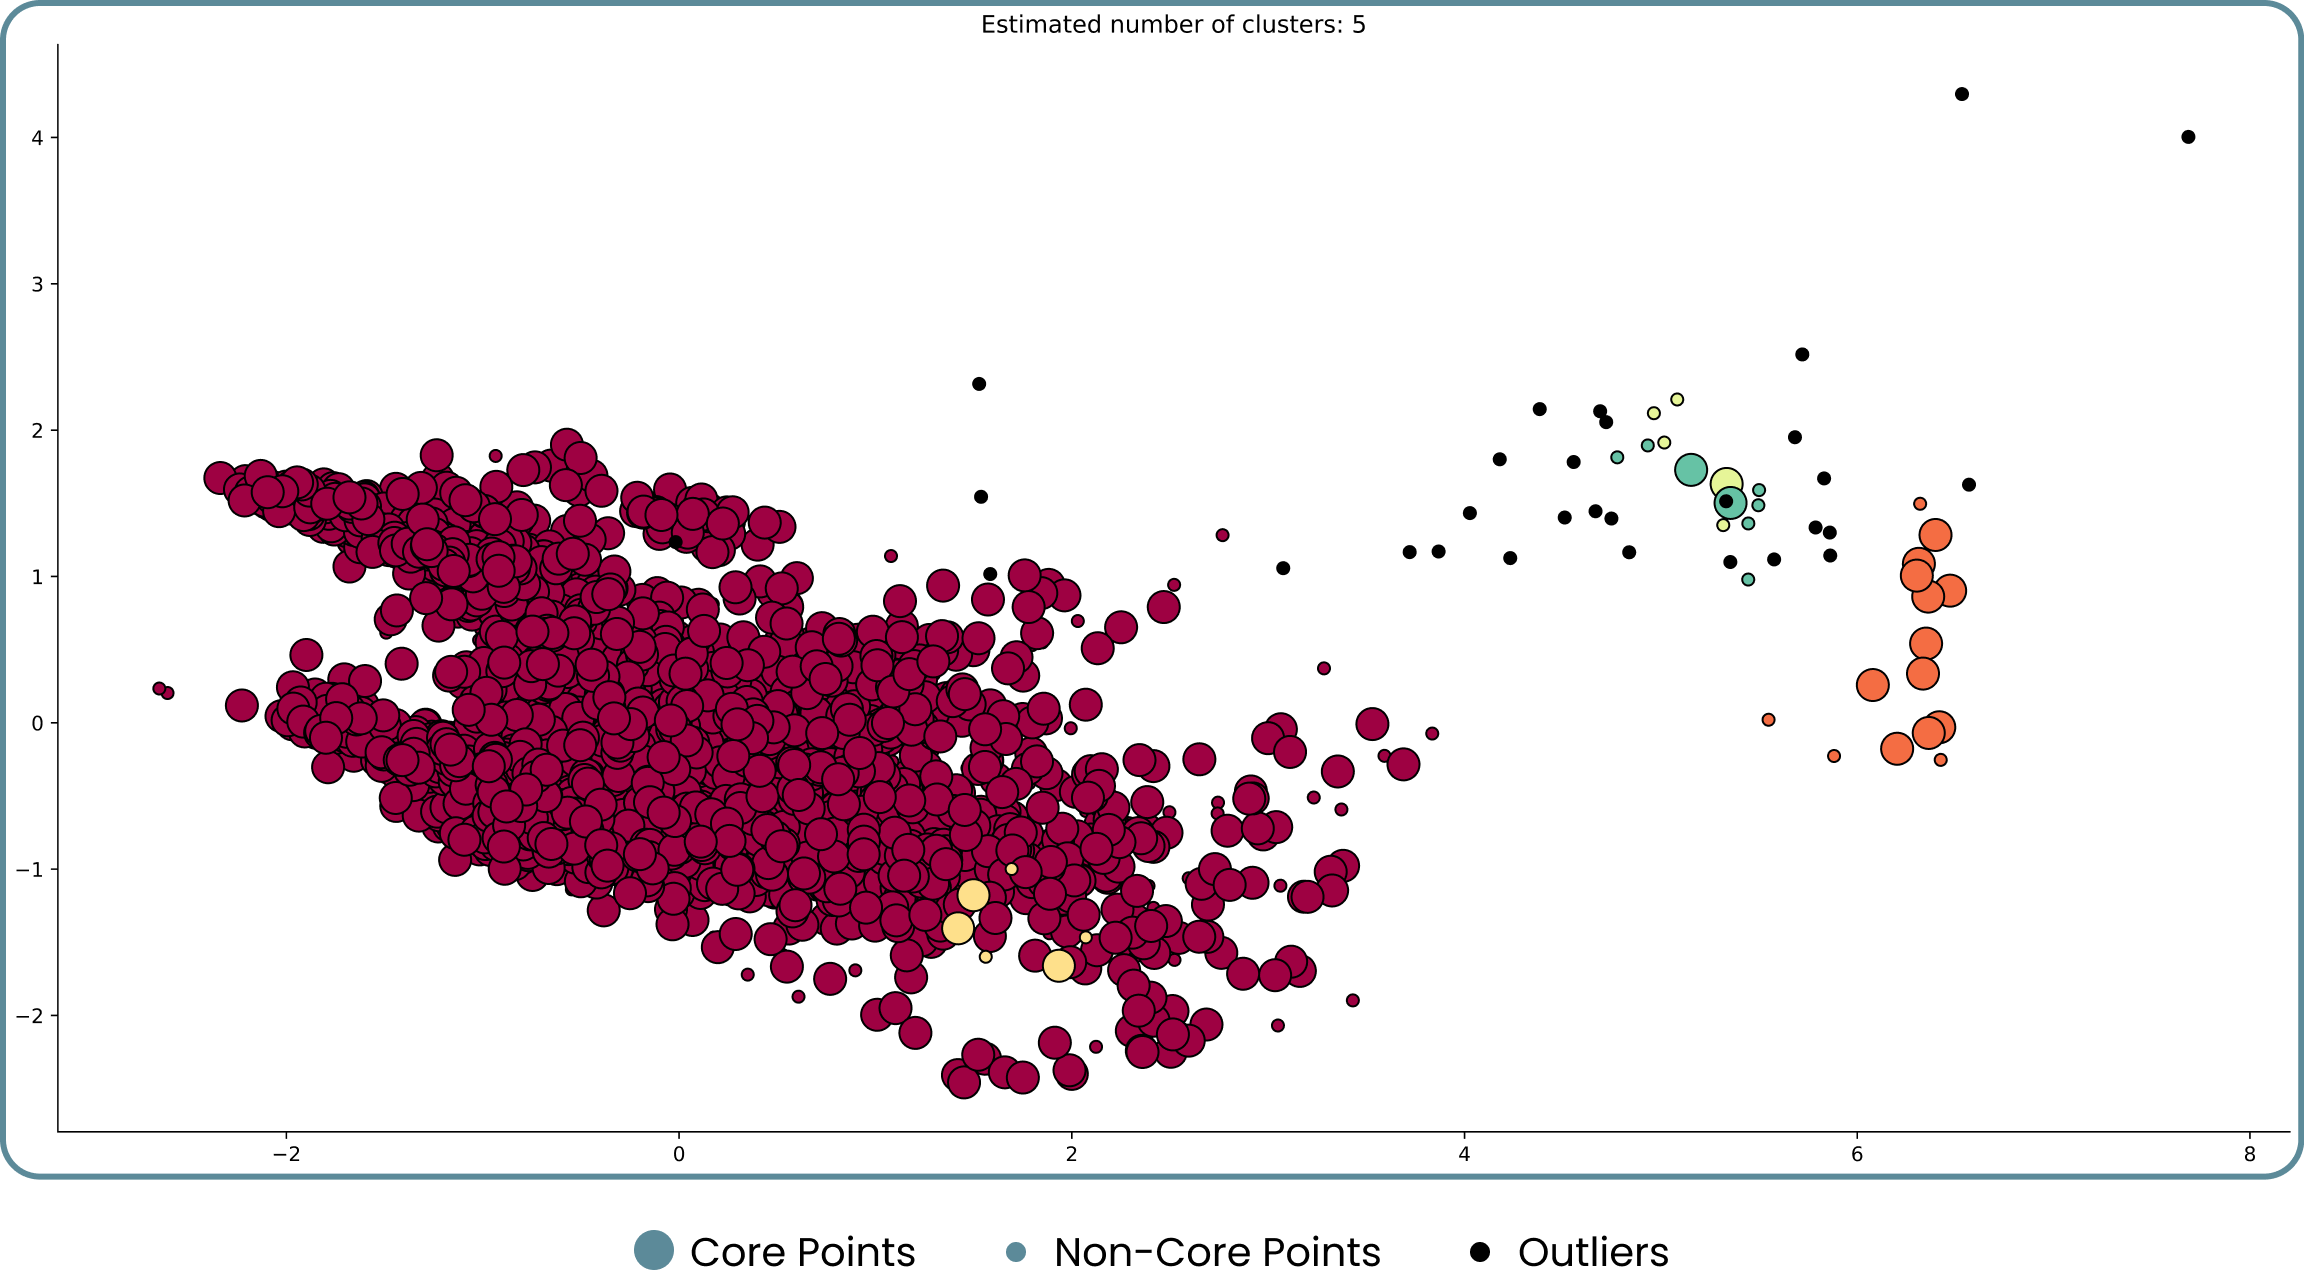
\includegraphics[width=13cm]{Images/3/clusters.png}
    \caption{Graphic representation of clusters in 2 components with PCA}
    
    
\end{figure}